\documentclass{article}
\usepackage{setspace}
\usepackage{amsmath}
\usepackage{graphicx}
\usepackage{float}
\usepackage{subcaption}
% This is gonna give you footnote
% \usepackage[backend=bibtex,style=verbose-trad2]{biblatex}
% And this is gonna give you some collection
\usepackage[backend=bibtex,style=ieee]{biblatex}
\usepackage{siunitx} % Required for alignment
\usepackage{multirow}
\usepackage{booktabs} % For prettier tables
\usepackage{longtable} % To display tables on several pages
\usepackage{rotating} % To display tables in landscape
\usepackage{pgfplotstable} % Generates table from .csv
\usepackage{tikz}
\usepackage{pgfplots}
\usepackage{csvsimple}
\usepackage{listings}
\usepackage[utf8]{inputenc}
% Well guess you need this to make sure line break of minted listing is working fine
\usepackage[newfloat]{minted}
% \usepackage{caption}

% You can change the style for minting here
% \usemintedstyle{vs}
\setminted{
    linenos=true,
    autogobble,
    breaklines=true,
}
\sisetup{
  round-mode          = places, % Rounds numbers
  round-precision     = 2, % to 2 places
}

\pgfplotsset{compat=newest}
\usepgfplotslibrary{units}
\title{Latex}
\date{2020-02-29}
\author{dendenxu}
\bibliography{welcome}

% Note that you can set the counter everywhere around the article so that some subsections show while others don't.
% \setcounter{tocdepth}{1} % Show sections
% \setcounter{tocdepth}{2} % + subsections
\setcounter{tocdepth}{3} % + subsubsections
%\setcounter{tocdepth}{4} % + paragraphs
% \setcounter{tocdepth}{5} % + subparagraphs

\begin{document}
\maketitle
\pagenumbering{gobble}

\newpage
\doublespacing
\tableofcontents
\singlespacing


\newpage
\pagenumbering{arabic}

\section{Section}
Hello, world.
\subsection{Subsection}
Structuring a document is easy.
\subsubsection{Subsubsection}
\paragraph{Paragraph}

Some more text.

\subparagraph{Subparagraph}

Even more text.

\section{Another section}

\begin{equation}
    f(x) = x^2
\end{equation}

% This is going to create equations without numbers
\begin{equation*}
    f(x) = x^2
\end{equation*}

This formula is an equation. $f(x) = ax^2+bx+c$

\begin{equation*}
    a + b = c
\end{equation*}
\begin{equation*}
    c + d = e
\end{equation*}

\begin{align*}
    a + b & = c     \\
    c     & = d + e
\end{align*}

\begin{align*}
    f(x) & = x^2                     \\
    g(x) & = \frac{1}{x}             \\
    F(x) & = \int^a_b \frac{1}{3}x^3
\end{align*}

% Well, this is new
\begin{align*}
    \begin{matrix}
        1 & 0 \\
        0 & 1
    \end{matrix}
\end{align*}

\begin{align*}
    \left[
        \begin{matrix}
            1 & 0 \\
            0 & 1
        \end{matrix}
        \right]
\end{align*}

\paragraph{Extra Paragraph}

This is for splitting the pages.

\section{Photo And Figure}

% This h is making the image here, and the ! forces it
\begin{figure}[!ht]
    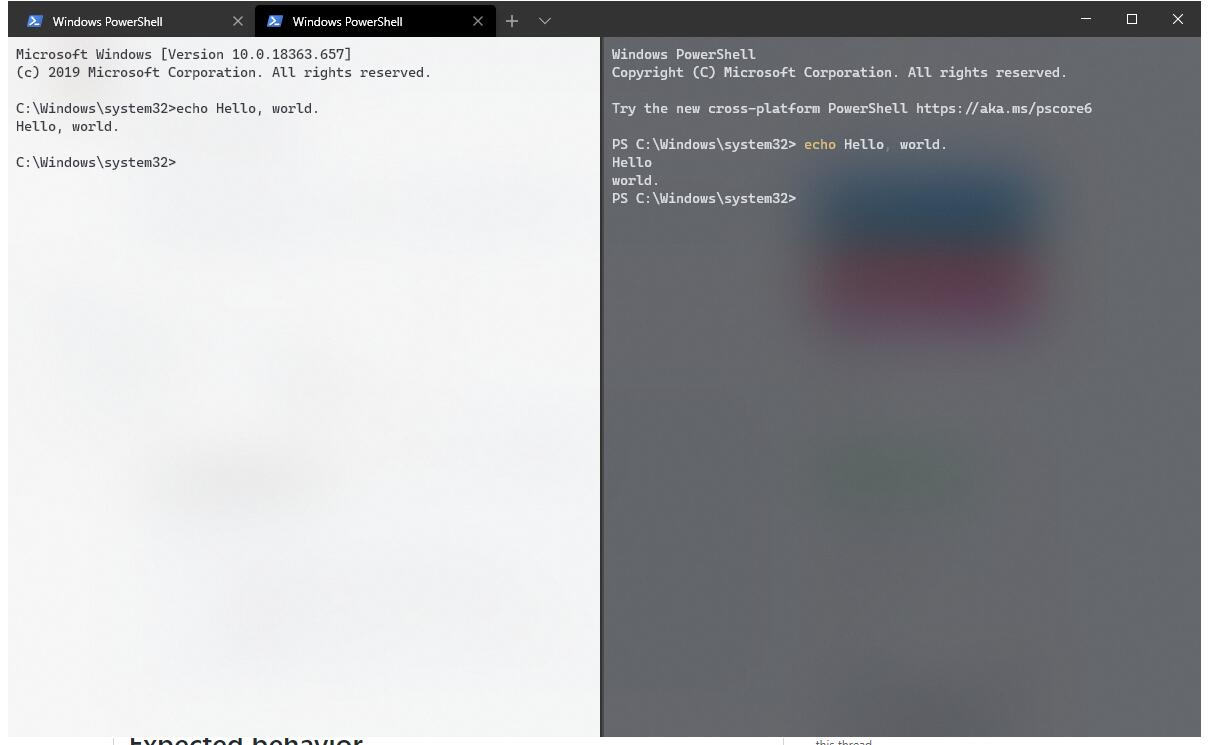
\includegraphics[width=\linewidth]{echos.jpg}
    \caption{A Windows Terminal.}
    \label{fig:Terminal}
\end{figure}
\section{Another another section}
\paragraph{Wow}
Figure \ref{fig:Terminal} shows a split terminal.


\begin{figure}[!ht]
    % This is gonna center this image elegantly
    \centering
    \begin{subfigure}[b]{0.4\linewidth}
        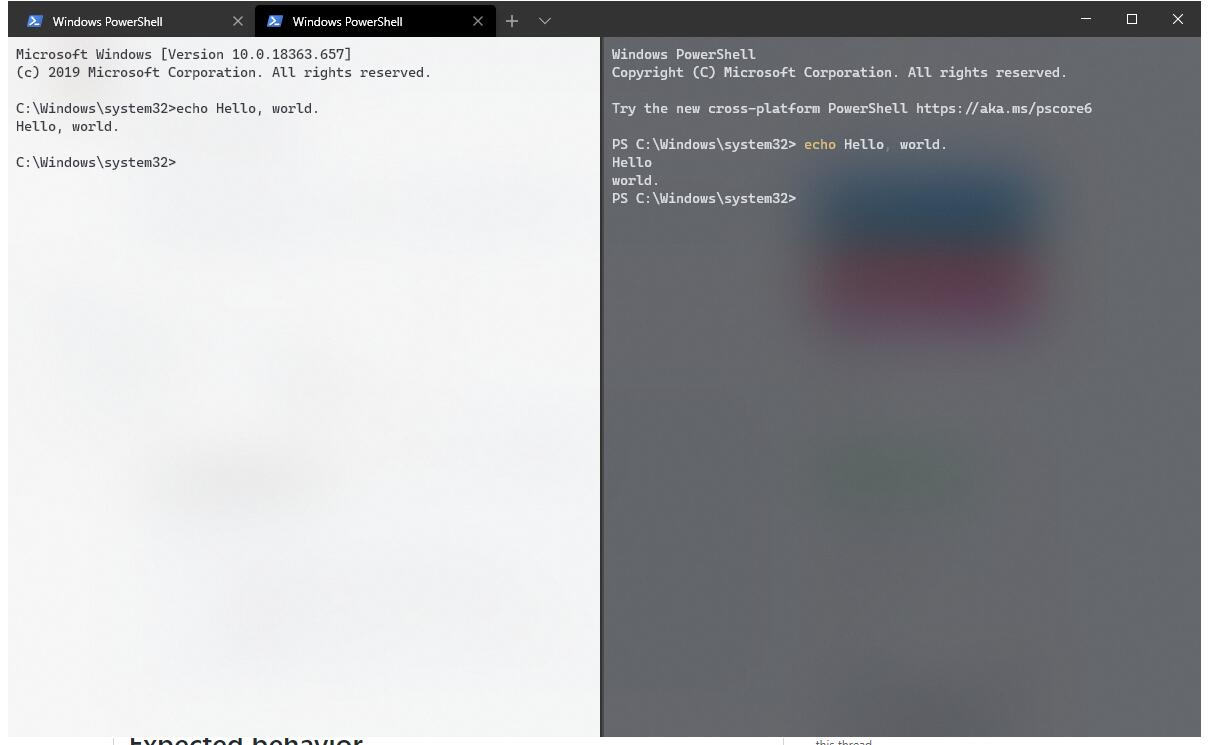
\includegraphics[width=\linewidth]{echos.jpg}
        \caption{An Echo}
    \end{subfigure}
    \begin{subfigure}[b]{0.4\linewidth}
        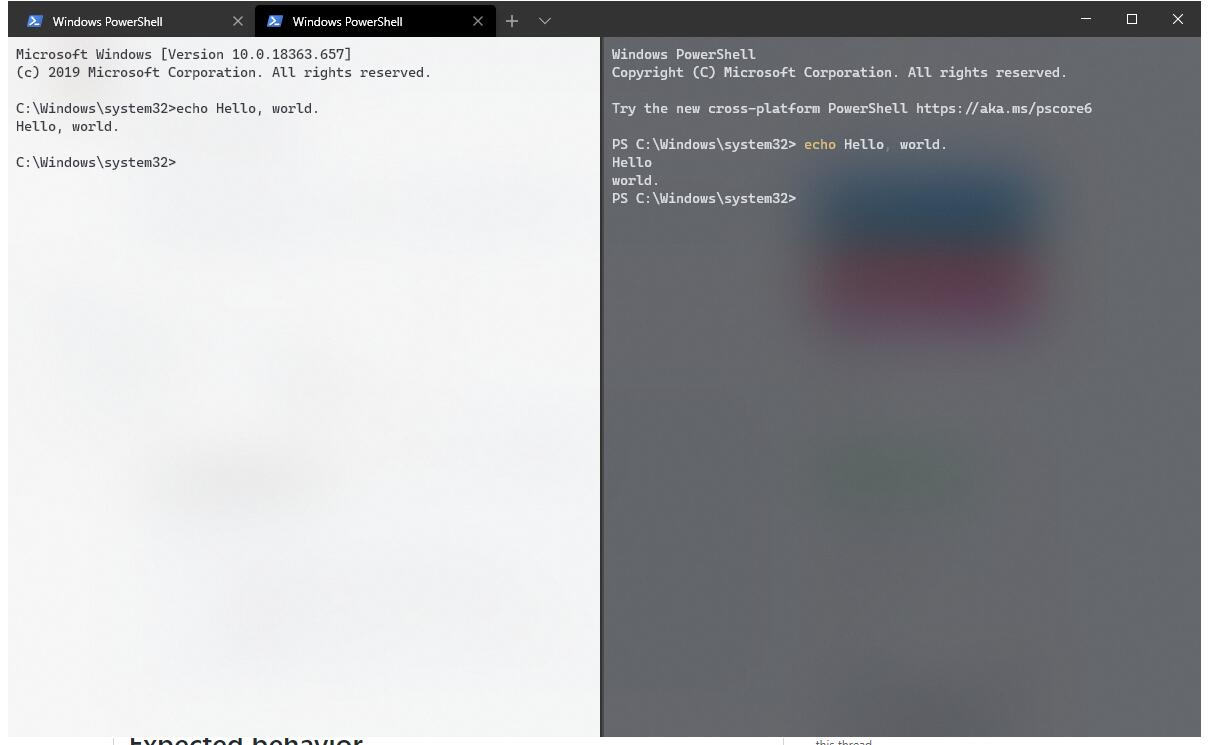
\includegraphics[width=\linewidth]{echos.jpg}
        \caption{Another Echo}
    \end{subfigure}
    \caption{Two Terminal, Four Echos}
    \label{fig:TwoTerminal}
\end{figure}

\begin{figure}[!ht]
    \caption{Dummy Figure}
\end{figure}

\begin{table}[!ht]
    \caption{Dummy Table No.0}
\end{table}


\newpage
\section{Try Using BibTex}

This is a random citation \autocite{LeeRice-4} here.
% This is a random citation \cite{LeeRice-4} here.
And this would be another citation: \autocite{AragonRios-30}.
% And this would be another citation: \cite{AragonRios-30}.
Here's another \autocite{Starobin-32} one.
% Here's another \cite{Starobin-32} one.

\subsection{Footnote}
% If you use BibLaTex you may also use the default footnote of latex
Random citation \autocite{LeeRice-4} embedded in text.
This is some example text\footnote{\label{myfootnote}Hello footnote}.

\subsection{Refer to Footnote}
I'm referring to footnote \ref{myfootnote}.

\section{Drawing Tables}
Sometimes we use what's already given in latex to elegantly draw some tables. They may look more "academic" if you compare it with excel or other tools.

\subsection{Ordinary Table}
This would be an ordinary little table for us to use. Multiple fun stuff like multi-row and multi-column can come in handy when doing customization.

\begin{table}[!ht]
    % Turns out you'll have to add a center environment huh
    \begin{center}
        \caption{First Table}
        % Don't know why, you HAVE TO PUT DOUBLE SLASH IN LONG TABLE
        % AND YOU CANNNOT DO THE SAME WITH THIS TABULAR BAR
        \label{tab:Table1}
        \begin{tabular}{l|S|r}
            \toprule
            \textbf{Value1}                            & \textbf{Value2} & \textbf{Value3} \\
            $\alpha$                                   & $\beta$         & $\gamma$        \\
            \midrule
            \multicolumn{2}{c|}{12}                    & a                                 \\ % <-- Combining two cells with alignment c| and content 12.
            \hline
            \multirow{2}{*}{12}                        & 1110.1          & a               \\ % <-- Combining 2 rows with arbitrary with (*) and content 12
                                                       & 10.1            & b               \\ % <-- Content of first column omitted.
            \hline
            \multicolumn{2}{c|}{\multirow{2}{*}{1234}} & a                                 \\ % <-- Multicolumn spanning 2 columns, content multirow spanning two rows
            \multicolumn{2}{c|}{}                      & b                                 \\ % <-- Multicolumn spanning 2 columns with empty content as placeholder
            \hline
            1                                          & 1100.1          & a               \\
            3                                          & 11.1            & b               \\
            5                                          & 10.112          & v               \\
            \bottomrule
        \end{tabular}
    \end{center}
\end{table}

\subsection{Longtable}
This guy here has the ability to cross multiple page if its too large to fit in one page. However when it comes to the ordinary one, the information would just be truncated.
What's the overhead of using such multi-page table?
Probably it's that you have to specify two kinds of header for both the original and next-page version of our table.

\paragraph{Ramdom Figure}
Let's add some random figure so that we may see the magic of long table.

\begin{figure}[!ht]
    % This is gonna center this image elegantly
    \centering
    \begin{subfigure}[b]{0.4\linewidth}
        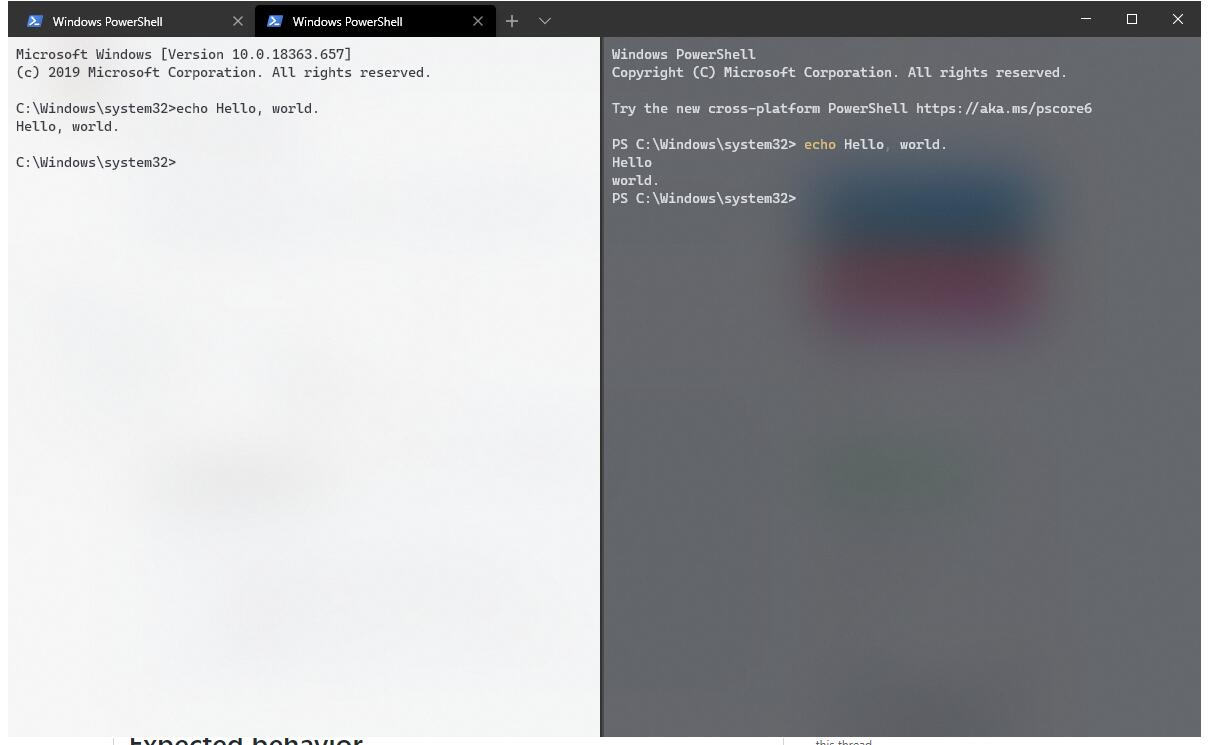
\includegraphics[width=\linewidth]{echos.jpg}
        \caption{An Echo}
    \end{subfigure}
    \begin{subfigure}[b]{0.4\linewidth}
        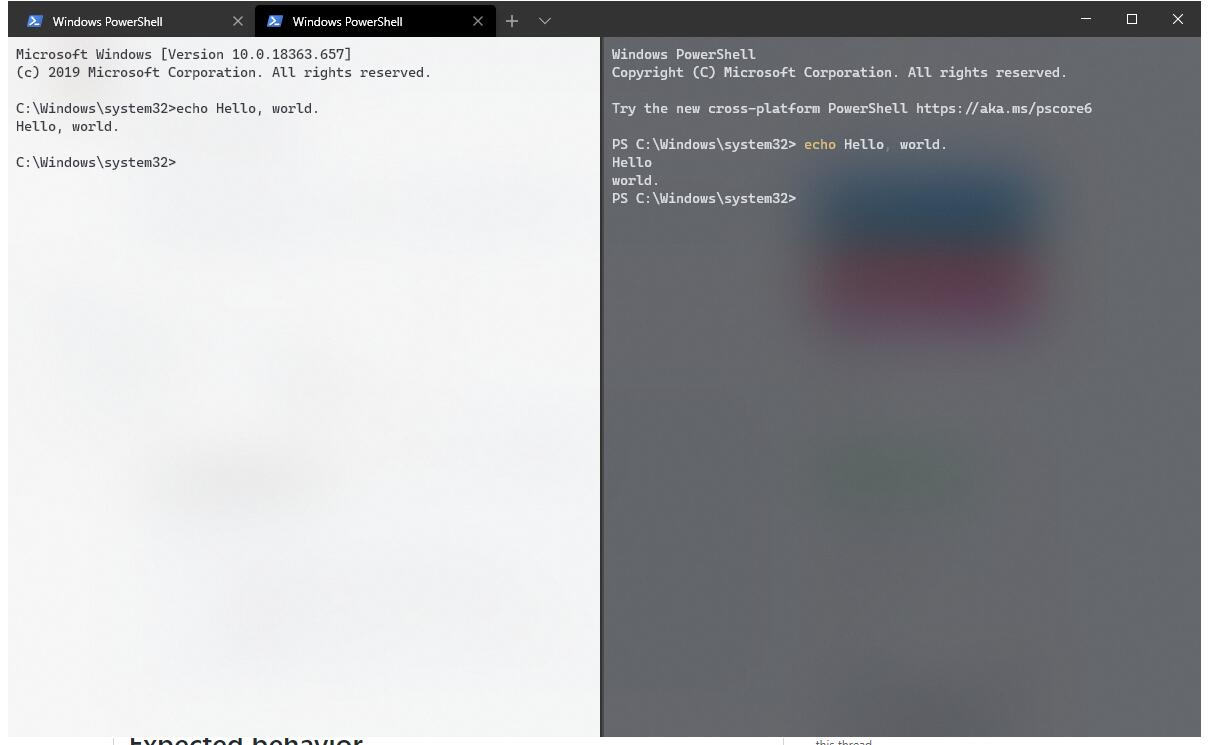
\includegraphics[width=\linewidth]{echos.jpg}
        \caption{Another Echo}
    \end{subfigure}
    \caption{Two Terminal, Four Echos}
    \label{fig:TwoTerminal_random2}
\end{figure}

\begin{figure}[!ht]
    % This is gonna center this image elegantly
    \centering
    \begin{subfigure}[b]{0.4\linewidth}
        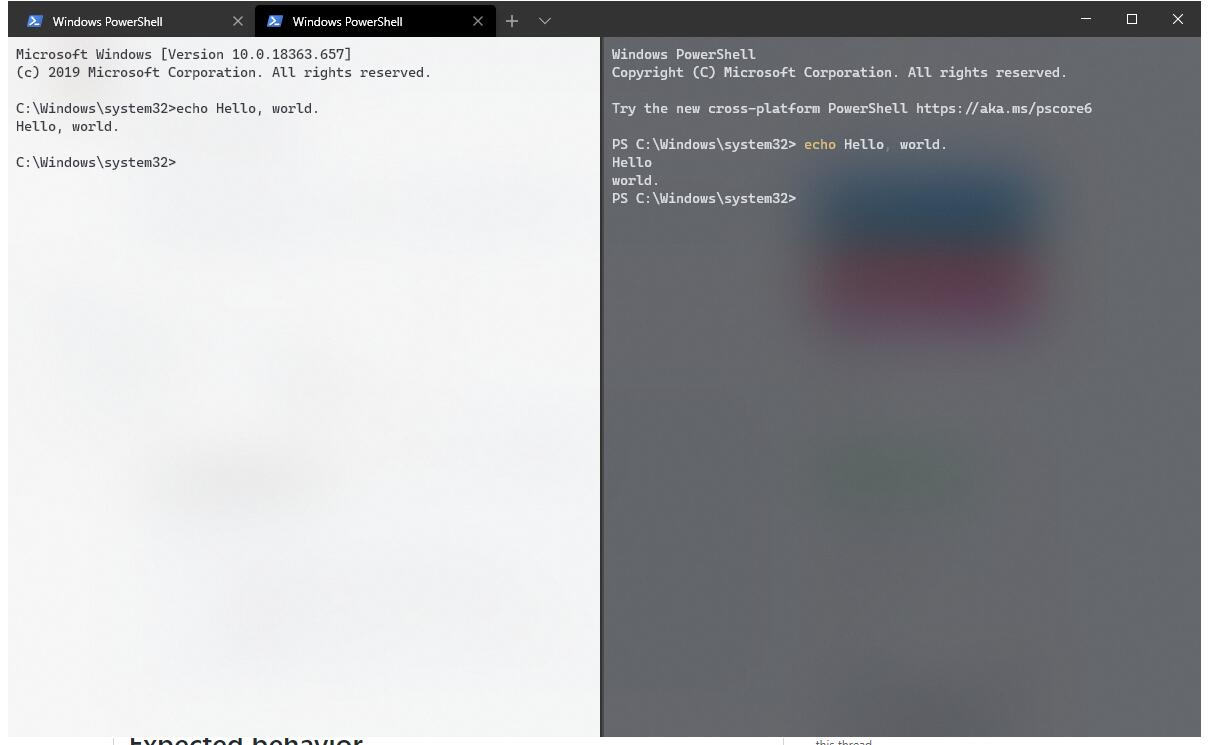
\includegraphics[width=\linewidth]{echos.jpg}
        \caption{An Echo}
    \end{subfigure}
    \begin{subfigure}[b]{0.4\linewidth}
        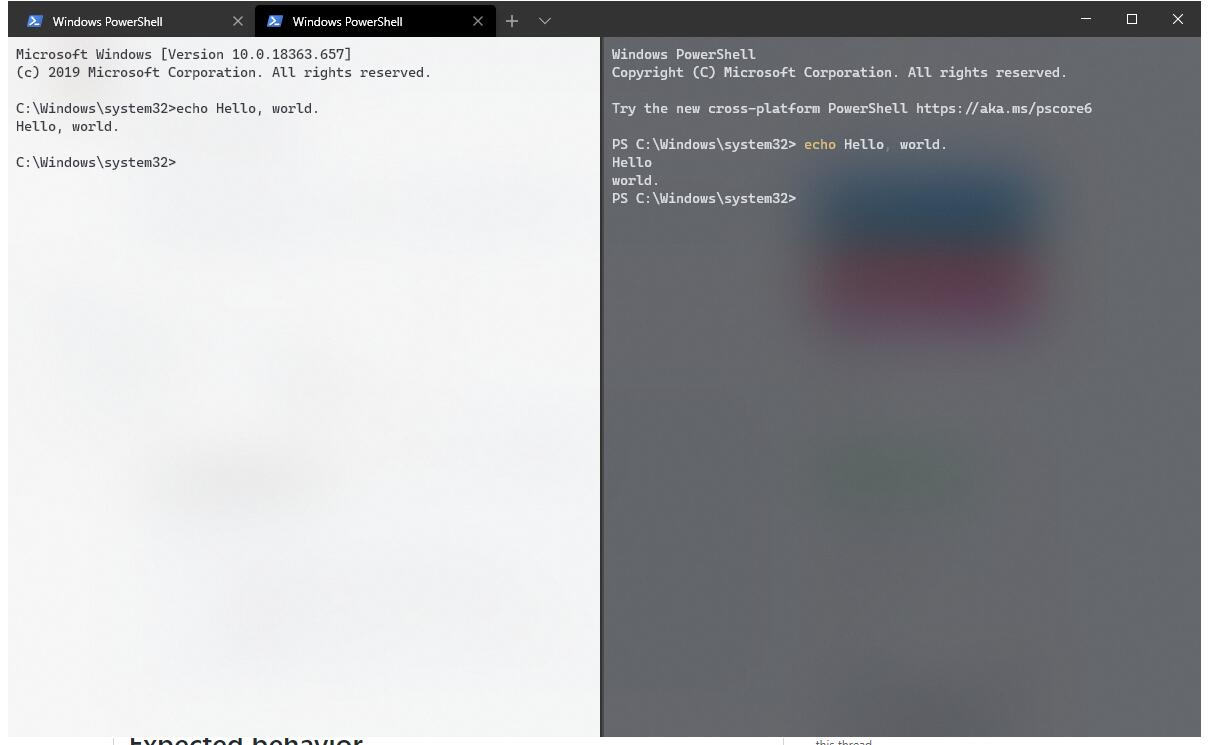
\includegraphics[width=\linewidth]{echos.jpg}
        \caption{Another Echo}
    \end{subfigure}
    \caption{Two Terminal, Four Echos}
    \label{fig:TwoTerminal_random1}
\end{figure}


\begin{longtable}[c]{l|S|r} % <-- Replaces \begin{table}, alignment must be specified here (no more tabular)
    \caption{Multipage table.}
    % I DON'T KNOW WHY SHOULD A LABEL END WITH THIS??
    % AND THE COMPILER JUST STUCK THERE?
    % WHAT THE HECK?
    % PROBLEM TEMPORARILY SOLVED BY ADDING THESE TWO SLASH
    \label{tab:Longtable}                                  \\
    \toprule
    \textbf{Value 1} & \textbf{Value 2} & \textbf{Value 3} \\
    $\alpha$         & $\beta$          & $\gamma$         \\
    \midrule
    \endfirsthead % <-- This denotes the end of the header, which will be shown on the first page only
    \toprule
    \textbf{Value 1} & \textbf{Value 2} & \textbf{Value 3} \\
    $\alpha$         & $\beta$          & $\gamma$         \\
    \midrule
    \endhead % <-- Everything between \endfirsthead and \endhead will be shown as a header on every page
    1                & 1110.1           & a                \\
    2                & 10.1             & b                \\
    % ...
    % ... Many rows in between
    % ...
    3                & 23.113231        & c                \\
    3                & 23.113231        & c                \\
    3                & 23.113231        & c                \\
    3                & 23.113231        & c                \\
    3                & 23.113231        & c                \\
    \bottomrule
\end{longtable}


\subsection{Dummy Figure}
Let's fill in the space again.

\begin{figure}[!ht]
    \centering
    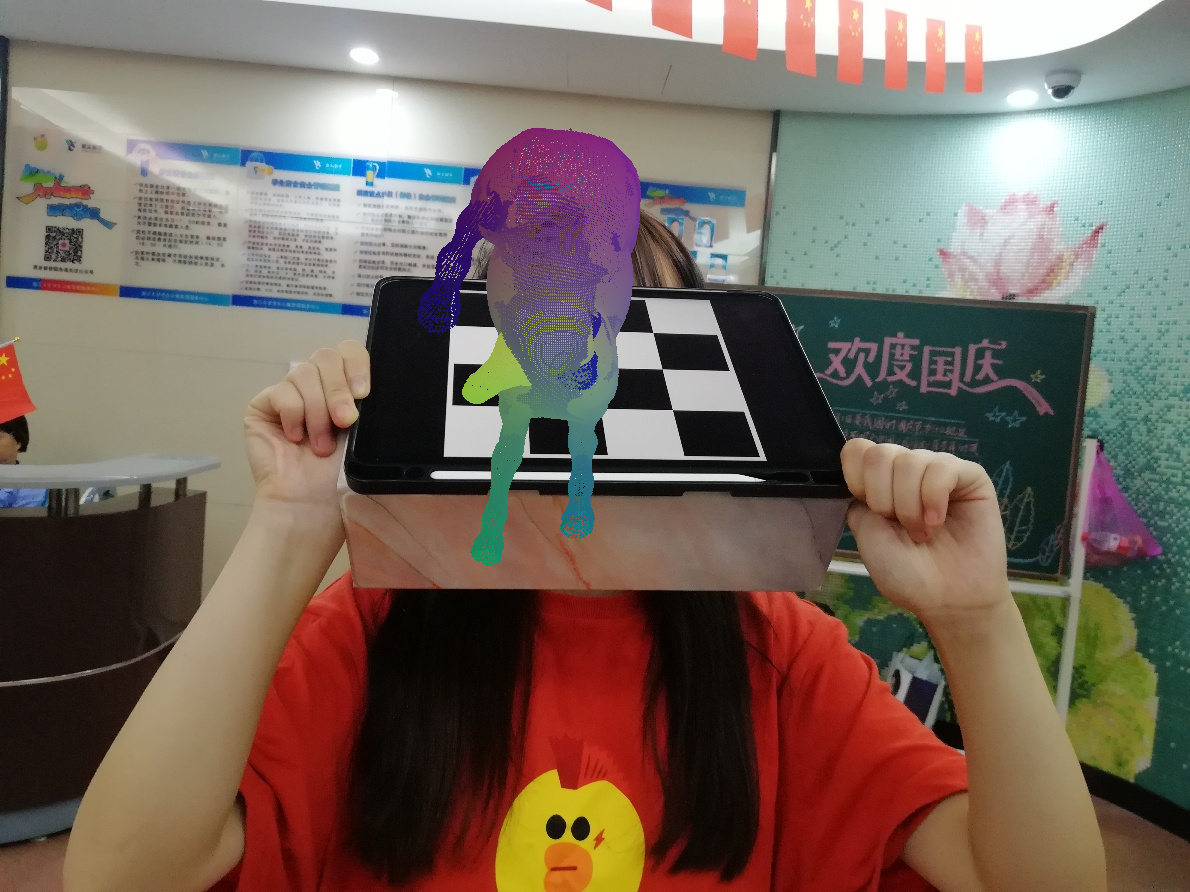
\includegraphics[width=0.8\linewidth]{3_horse.png}
    \caption{See! A horse!}
    \label{fig:horse}
\end{figure}

% Don't know why,
% When you try to use sidewaystable or landscape table
% The use of float can get really messy
% When you use [!ht], the table might just go to the end of the file
% And when you omit it, it appears right here
% heheda
\subsection{Sideways Table}
Well, guess the floating implementation of such sideways table isn't perfect. Like I've talked about in the previous comment, you use [!h] and the table goes to somewhere strange. When you omit it, table gets back magically.
Boy, it's magic.
\begin{sidewaystable} % <--
    \begin{center}
        \caption{Landscape table.}
        \label{tab:table1}
        \begin{tabular}{l|S|r|r|r|r}
            \toprule
            \textbf{Value 1} & \textbf{Value 2} & \textbf{Value 3} & \textbf{3} & \textbf{4} & \textbf{5} \\
            $\alpha$         & $\beta$          & $\gamma$         & $\gamma$   & $\gamma$   & $\gamma$   \\
            \midrule
            1                & 1110.1           & a                & a          & a          & a          \\
            2                & 10.1             & b                & b          & b          & b          \\
            3                & 23.113231        & c                & c          & c          & c          \\
            3                & 23.113231        & c                & c          & c          & c          \\
            3                & 23.113231        & c                & c          & c          & c          \\
            3                & 23.113231        & c                & c          & c          & c          \\
            3                & 23.113231        & c                & c          & c          & c          \\
            3                & 23.113231        & c                & c          & c          & c          \\
            3                & 23.113231        & c                & c          & c          & c          \\
            3                & 23.113231        & c                & c          & c          & c          \\
            3                & 23.113231        & c                & c          & c          & c          \\
            3                & 23.113231        & c                & c          & c          & c          \\
            3                & 23.113231        & c                & c          & c          & c          \\
            3                & 23.113231        & c                & c          & c          & c          \\
            3                & 23.113231        & c                & c          & c          & c          \\
            3                & 23.113231        & c                & c          & c          & c          \\
            3                & 23.113231        & c                & c          & c          & c          \\
            \bottomrule
        \end{tabular}
    \end{center}
\end{sidewaystable}

\newpage
\subsection{Gimme CSV}
Wow, so, you can export figures out of excel and other tools in a CSV file(line break), and the file can be easily imported as a plot.

\begin{table}[!ht]
    \caption{Auto generated table for csv file.}
    \label{tab:csv}
    \begin{center}
        \pgfplotstabletypeset[
            col sep=comma,
            multicolumn names, % allows to have multicolumn names
            % It seems that you'll print everything in the CSV file here
            % But you can use the following lines to specify individual format 
            display columns/0/.style={
                    column type={S}, string type,
                },
            display columns/1/.style={
                    column type={S}, string type,
                },
            display columns/4/.style={
                    column type={S}, string type,
                },
            display columns/5/.style={
                    column type={S}, string type,
                },
            every head row/.style={{before row=\toprule},{after row=\midrule}},
            every last row/.style={after row=\bottomrule},
        ]{hello.csv}
        % \pgfplotstabletypeset[
        % multicolumn names, % allows to have multicolumn names
        % col sep=comma, % the seperator in our .csv file
        % display columns/0/.style={
        %         column name=$A$, % name of first column
        %         column type={S},string type},  % use siunitx for formatting
        % display columns/1/.style={
        %         column name=$B$,
        %         column type={S},string type},
        % display columns/2/.style={
        %         column name=$B$,
        %         column type={S},string type},
        % every head row/.style={before row={\toprule},}, % have a rule at top 
        % every last row/.style={after row=\bottomrule}, % rule at bottom
        % ]{hello.csv} % filename/path to file
    \end{center}
\end{table}

\begin{table}[!ht]
    \caption{Related to the figure, using pgfplots}
    \label{tab:figure}
    \begin{center}
        \pgfplotstabletypeset[
            col sep=comma, % Wow this is the magic line
            every head row/.style={{before row=\toprule},{after row=\midrule}},
            every last row/.style={after row=\bottomrule},
        ]{123.csv}
    \end{center}
\end{table}

% \begin{table}[H]
%     \begin{longtable}{lr}
%         \caption{This is created using csvsimple}
%         \label{tab:CSVSIMPLE_aha}             \\
%         \toprule
%         \bfseries x             & \bfseries y \\
%         \midrule
%         \endhead
%         \bottomrule
%         \endfoot
%         \csvreader[
%             late after line=                  \\,
%             late after last line=,
%             after reading={\bottomrule}
%         ]
%         {123.csv}{1=\x,2=\y}{\x & \y}
%     \end{longtable}
% \end{table}

\subsection{Oneline CSV}
Or we can just use the one line version right?
Do remember to add [H].
\begin{table}[H]
    \begin{center}
        \caption{One line csv}
        \label{tab:oneline}
        \csvautobooktabular{hello.csv}
    \end{center}
\end{table}

\csvautobooklongtable[
    table head=\caption{some table}\label{tab:some}\\\hline
    \csvlinetotablerow\\\midrule
    \endfirsthead\hline
    \csvlinetotablerow\\\midrule
    \endhead\bottomrule
    \endfoot,
]{hello.csv}

\subsection{Plot From CSV}

% I f**king hate the error log of tex compiler
\begin{figure}[H]
    \begin{center}
        \caption{My first auto-generated plot.}
        \begin{tikzpicture}
            \begin{axis}[
                    width=\linewidth, % Scale the plot to \linewidth
                    grid=major, % Display a grid
                    grid style={dashed,gray!30}, % Set the style
                    xlabel=X Axis $U$, % Set the labels
                    ylabel=Y Axis $I$,
                    x unit=\si{\volt}, % Set the respective units
                    y unit=\si{\ampere},
                    legend style={at={(0.5,-0.2)},anchor=north}, % Put the legend below the plot
                    x tick label style={rotate=90,anchor=east} % Display labels sideways
                ]
                \addplot
                % add a plot from table; you select the columns by using the actual name in
                % the .csv file (on top)
                table[x=x,y=y,col sep=comma] {123.csv};
                \legend{Plot}
            \end{axis}
        \end{tikzpicture}
    \end{center}
\end{figure}

\subsection{Draw lines by hand}
Well, well, well.
When you want to make sure something is where you want it to be, you can simply use [H] with the support of package {float}.

\begin{figure}[H]
    \caption{Some self drawn figure}
    \label{fig:handmade}
    \begin{center}
        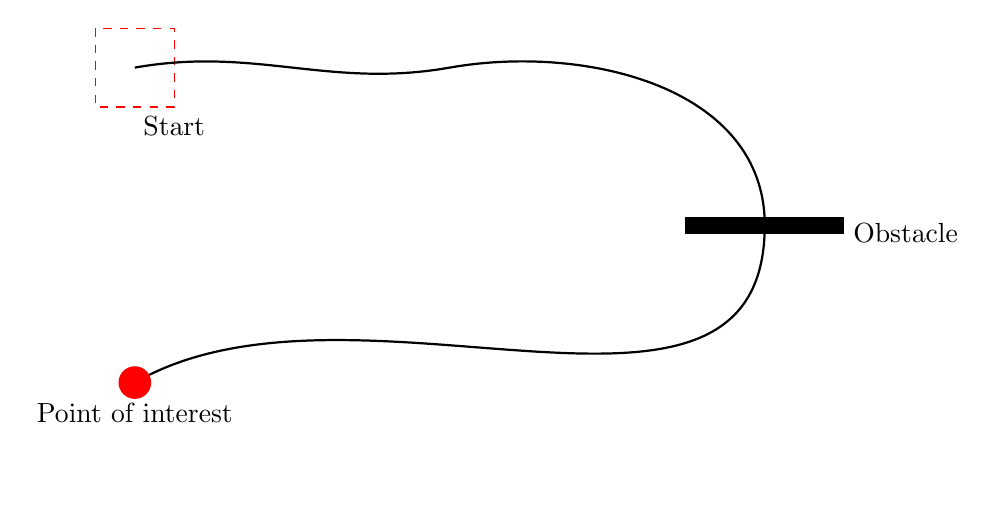
\begin{tikzpicture}
            % You can always use draw to add new stuff on this floating section
            \draw [red,dashed] (-2.5,2.5)
            rectangle (-1.5,1.5)
            node [black,below] {Start}; % Draws a rectangle

            \draw [thick] (-2,2) % Draws a line
            to [out=10,in=190] (2,2)
            to [out=10,in=90] (6,0)
            to [out=-90,in=30] (-2,-2);

            \draw [fill] (5,0.1)
            rectangle (7,-0.1)
            node [black,right] {Obstacle}; % Draws another rectangle

            \draw [red,fill] (-2,-2)
            circle [radius=0.2]
            node [black,below=4] {Point of interest}; % Draws a circle

        \end{tikzpicture}
    \end{center}
\end{figure}

\section{Code}
\subsection{Default stuff}
We can use verbatim as the default code displayer. It won't highlight keywords or emphasis.

\begin{verbatim}
Text listed here will be printed using mono-space font.
Text listed here will be printed using mono-space font.
Text listed here will be printed using mono-space font.
Text listed here will be printed using mono-space font.
Text listed here will be printed using mono-space font.
Text listed here will be printed using mono-space font.
Text listed here will be printed using mono-space font.
\end{verbatim}

\begin{verbatim*}
    Or we can use star to indicate that we want to render white space.
    Text listed here will be printed using mono-space font.
    Text listed here will be printed using mono-space font.
    Text listed here will be printed using mono-space font.
    Text listed here will be printed using mono-space font.
    Text listed here will be printed using mono-space font.
    Text listed here will be printed using mono-space font.
\end{verbatim*}

\subsection{lstlisting}
Trying to list we emphasis.
Well, I don't think I'm gonna use this more than we should.
Since the mindted package looks much much better.
\lstset{
    basicstyle=\ttfamily,
    columns=fullflexible,
    frame=single,
    breaklines=true,
    postbreak=\mbox{\textcolor{red}{$\hookrightarrow$}\space},
}
\begin{listing}[H]
    \caption{Listing Using lstlisting}
    \begin{lstlisting}[language=c++]
bool MIPSAssembler::CheckLineEnd(stringstream &str_stream)
{
    Trim(str_stream, ' ');
    if (str_stream.peek() == '#' || str_stream.peek() == '\n') {
        DiscardLine(input);
        return true;
    } else if (str_stream.peek() == '\r') {
        if (!Linux_warning) {
            Linux_warning = true;
            cerr << "WARNING: Processing CRLF file on Linux system." << endl;
        }
        str_stream.get();
        if (str_stream.peek() != '\n') {
            cerr << "FATAL: Carrige Return encountered, however no Line Feed is found, file corrupted." << endl;
            return false;
        }
        DiscardLine(input);
        return true;
    } else if (str_stream.peek() != EOF) {
        cerr << "FATAL: Unexpected line end." << endl;
        return false;
    } else
        return true;
}
    \end{lstlisting}
\end{listing}


\subsection{List With Minted}
% Create a new environment for breaking code listings across pages.
\newenvironment{longlisting}{\captionsetup{type=listing}}{}
\begin{longlisting}
    \caption{List with minted.}
    \begin{minted}[breaklines,frame=single,linenos]{cpp}
bool MIPSAssembler::CheckLineEnd(stringstream &str_stream)
{
    Trim(str_stream, ' ');
    if (str_stream.peek() == '#' || str_stream.peek() == '\n') {
        DiscardLine(input);
        return true;
    } else if (str_stream.peek() == '\r') {
        if (!Linux_warning) {
            Linux_warning = true;
            cerr << "WARNING: Processing CRLF file on Linux system." << endl;
        }
        str_stream.get();
        if (str_stream.peek() != '\n') {
            cerr << "FATAL: Carrige Return encountered, however no Line Feed is found, file corrupted." << endl;
            return false;
        }
        DiscardLine(input);
        return true;
    } else if (str_stream.peek() != EOF) {
        cerr << "FATAL: Unexpected line end." << endl;
        return false;
    } else
        return true;
}
void MIPSAssembler::Trim(stringstream &str_stream, char ch)
{
    while (str_stream.get() == ch) // Will consume an extra character, so we put it back
        ;
    str_stream.unget();
}

bool MIPSAssembler::Assert(stringstream &str_stream, char ch)
{
    if (str_stream.get() == ch) return true; // Get next character an validate it
    cerr << "FATAL: Unable to read the character: " << ch << endl;
    return false;
}

bool MIPSAssembler::TrimAssert(stringstream &str_stream, char trim, char assert)
{
    Trim(input, trim);
    if (!Assert(str_stream, assert)) return false;
    Trim(input, trim);
    return true;
}

void MIPSAssembler::GetToken(stringstream &str_stream, string &str)
{
    str.clear();                                                                     // Clear string buffer
    while (!reserved_char.count(str_stream.peek())) str.push_back(str_stream.get()); // Get char if not reserved
}

bool MIPSAssembler::ReadConstant(stringstream &str_stream, int &constant)
{
    if ((str_stream >> constant)) return true; // Try interpreting the string into an integer
    cerr << "FATAL: Unable to read the constant." << endl;
    return false;
}

bool MIPSAssembler::ReadRegister(stringstream &str_stream, map<string, int>::iterator &reg_iter)
{
    string str;
    GetToken(input, str);

    // Return false if we cannot map the string to a register
    if ((reg_iter = reg_map.find(str)) != reg_map.end()) return true;
    cerr << "FATAL: Unable to map register: " << str << " to int value." << endl;
    return false;
}
void MIPSAssembler::DiscardLine(stringstream &str_stream)
{
    source_line_number++;
    while ((str_stream.get() != '\n') && (!str_stream.eof()))
        ;
}
    \end{minted}
\end{longlisting}

\newpage
\begin{appendix}
    \listoffigures
    \listoftables
    \listoflistings
    % \bibliographystyle{ieeetr}
    \printbibliography
\end{appendix}
\end{document}